\subsection{Cpp2UML}

Afin d'avoir un rapide aperçu du projet ainsi qu'une vision globale des différentes classes réalisées et de leurs dépendance,
nous avons tenté de générer un diagramme \textit{UML} de notre projet.

Un diagramme \textit{UML} est une façon de représenter le code de manière graphique.
Ce diagramme est composé d'une bulle, représentant une classe dans laquelle y est inscrite la liste des membres et attributs de cette classe avec des information de portée (privé, publique ...).
Chacune de ces bulles sont ensuite reliées entre elles par différentes flèches symbolisant les relations entre deux classes. Il est possible d'obtenir les information filiales, d'utilisation ou encore de contenance.

\begin{figure}[h!]
	\centering
	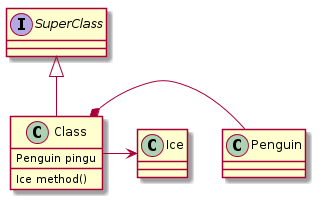
\includegraphics[width=0.8\textwidth]{img/uml_example.png}
	\caption{\textbf{Class} est une implementation d'une \textbf{SuperClass} qui utilise \textbf{Ice} et possède un \textbf{Penguin}, elle est composé d'un attribut \textit{pingu}, et d'une méthode \textit{surf}}
\end{figure}
\pagebreak
Dans le cadre de notre projet, nous avons réalisé un script en \textit{Lua},
permettant de générer automatiquement ce genre de graphique par le biais d'un autre outil:
\href{http://plantuml.sourceforge.net/}{PlantUML}.

Ce script annalyse les en-têtes de nos sources afin d'écrire un autre fichier de description compréhensible par PlantUML. Une fois ceci fait,  plantUML, en utilisant graphviz, crée une image de notre diagramme UML.
